%% This is the main content about this article. I should list them in an order
%% How to balance the existing model, positive and negative instance together, I shall use the dfg-method to create a dfg-matrix to incorporate the impact.
%% how to introduce them into adding long-term dependency feature. After mining the model by Inductive Miner, we have a model without long-term dependency, but we need to change the model and give the right examples.. 
%% If we change the data set, then we need to change the model into another parts, but the current methods can not solve it..
%% Should we also separate them into different sections?? Yes, we need it
%% Also, to delete the silent transition, as one option feature in our methods, we only delete it, in this situation, which will not affect the model behavoirs.

%% Or we could organize the content in this way:
%%  -- put the whole structure ahead and put all that we want to talk
%%  -- list the steps 
%%    ++ dfg-method to balance the directly-follows relation and create the corresponding directly-follows graph
%%    ++ add long-term dependency on the model
%%    ++ delete the silent transitions on the model as a post model

%% Put some words here
This chapter describes the repair algorithm to incorporate the negative instances on process enhancement. At the beginning, the main architecture is listed to provide an overview of our strategy. Main modules of the algorithm are described in the next sections. Firstly, the impact of the existing model, positive and negative instances are balanced in the media of the directly-follow relations. Inductive Miner is then applied to mine process models from those directly-follows relations. Again, we review the negative instances and express its impact by adding the long-term dependency. To add long-term dependency, extra places and silent transitions are created on the model, aiming to enforce the positive instances and block negative instances. Furthermore, the model in Petri net with long-term dependency can be  post-processed by reducing the silent transitions for the sake of simplicity.
\section{Architecture}
%% Describe the 
Figure \ref{fig:architecture} shows the steps of our strategy to enhance a process model. The basic inputs are an event log, and a Petri net. The traces in event log have an attribute for the classification labels of positive or negative in respect to some KPIs of business processes. The Petri net is the referenced model for the business process. To repair model with negative instances, the main steps are conducted.
\begin{figure}
	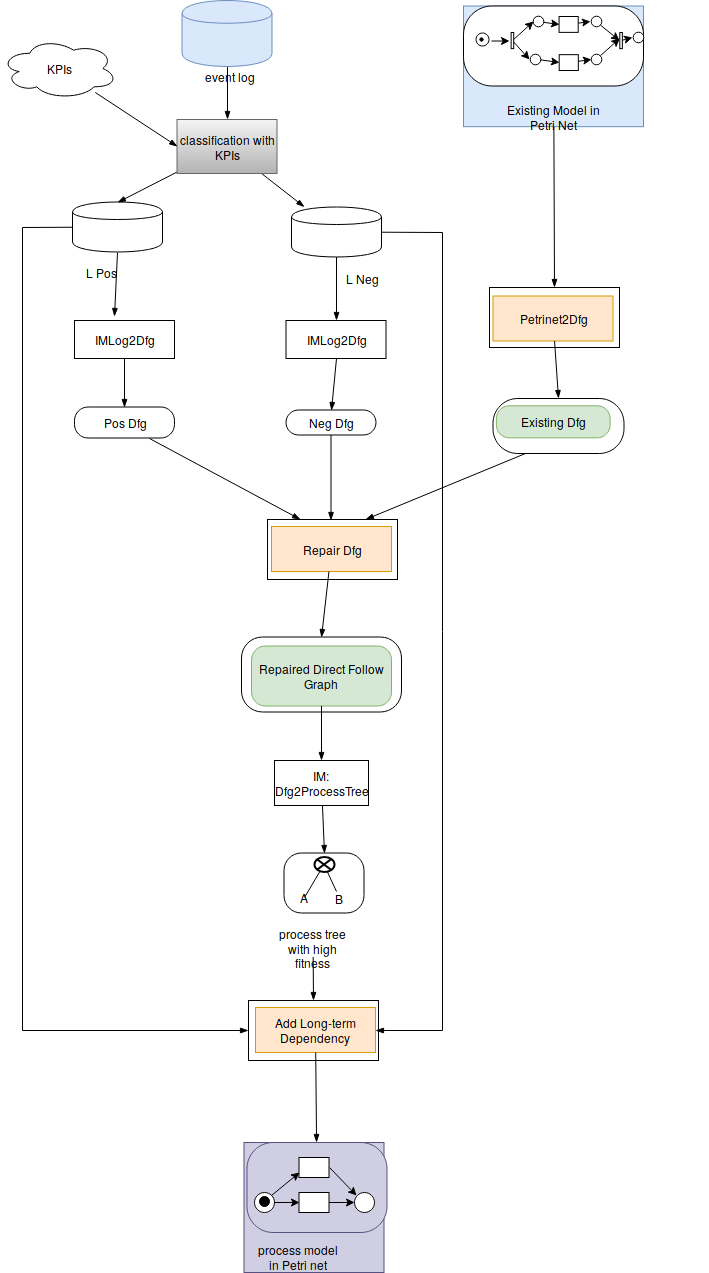
\includegraphics[width=0.9\textwidth, height=0.9\textheight]{figures/algorithm/FD_architecture_detail_02.png}
	\caption[Model Repair Architecture]{Model Repair Architecture -- \small Rectangles represents processes and output data in eclipse shape, especially customized processes and data are in doubled lattice shape. Input event log and existing model are in blue, KPIs are in cloud. The output is a petri net in purple. }
	\label{fig:architecture}
\end{figure} 
\begin{itemize}
	\item \emph{Generate directly-follows graph}\quad 
	Three directly-follows graph are generated respectively for the existing model, positive instance and negative instances from event log.
	\item \emph{Repair directly-follows graph} \quad
	The three directly-follows graphs are combined into one single directly-follows graph after balancing their impact.
	\item \emph{Mine models from directly-follows graph} \quad
	Process models are mined by Inductive Miner as intermediate results.
	\item \emph{Add long-term dependency} \quad
	Long-term dependency is detected on the intermediate models and finally added on the Petri net. To simplify the model, the reduction of silent transitions can be applied at end.
\end{itemize}
More details can be provided in the following sections.

\section{Generate directly-follows graph}
Originally, the even log $L$ is split into two sublogs, called $L_{pos}$ and $L_{neg}$. $L_{pos}$ contains the traces which is labeled as positive, while $L_{neg}$ contains the negative instances in the event log. Then, the two sublogs are passed to procedure \emph{IMLog2Dfg} to generate directly-follows graphs, respectively $G(L_{pos})$ and $G(L_{neg})$. More details about the procedure is available in \cite{leemans2013discovering}. 

To generate a directly-follows relation from  a Petri net, we gather the model behaviors by building a transitions system of its states. Then the directly-follows relations are extracted from state transitions. Based on those relations, we create a directly-follows graph for the existing model.

From the positive and negative event log, we can get the cardinality for corresponding directly-follows graph, to represent the strength of this directly-follows relation. However, when the existing model is transformed into  directly-follows graph $G(L_{ext})$, there is no point to assign cardinality on each edge. So we just set cardinality with 1 for each edge. 
\section{Repair directly-follows graph}
%% we can have subsection on it. How to repair on them??? 
To combine all information of the directly-follows graphs from the positive , negative instances and the existing model, namely $G(L_{pos})$, $G(L_{neg})$ and $G(L_{ext})$, the cardinality in directly-follows graphs is unified into the same range [0-1]. Since $G(L_{ext})$ is derived differently, its unified cardinality is based only on the given directly-follows graph and defined in the following. 
\begin{definition}[Unified cardinality for the existing Model]
Given a directly-follows graphs $G(L_{ext})$ for a model, the unified cardinality of each directly-follows relation is defined as \[ U_{ext}(E(A,B)) = \frac{Cardinality(E(A,B))}{Cardinality(E(A,*))}, with \]
	\[ Cardinality(E(A,*))=\sum{Cardinality(E(A,X) \vert E(A,X) \in G(L))}  \] 
	for start activities A, 
	\[ U(Start(A)) = \frac{Cardinality(Start(A))}{Cardinality(Start(*))} \]
	Similarly for end activities B,
	\[ U(End(B)) = \frac{Cardinality(End(B))}{Cardinality(End(*))} \]
$E(A,*)$ means all edges with source A, $E(*,B)$ means all edges with target B, $Start(*)$ represents all start nodes, and $End(*)$ represents all end nodes. 
\end{definition}
The unification of cardinality for positive and negative instances from an event log should consider the whole event log as its basic. 
\begin{definition}[Unified cardinality for $G(L_{pos})$, $G(L_{neg})$]
	Given a directly-follows graphs $G(L_{pos})$ for a model, the unified cardinality of each directly-follows relation is defined as 
	\begin{align*}
		&U_{pos}(E(A,B)) = \frac{Cardinality_{pos}(E(A,B))}{Cardinality(E(A,*))}, with  \\ 
		Cardinality(E(A,*))&=\sum{Cardinality_{pos}(E(A,X) + Cardinality_{neg}(E(A,Y))} where \\
		&	E(A,X) \in G(L_{pos}) and E(A,Y) \in G(L_{neg})) \\
		\text{for start activities A, } \\
		&U(Start_{pos}(A)) = \frac{Cardinality_{pos}(Start(A))}{Cardinality(Start(*))} \\
		\text{for end activities B,} \\
		&U(End_{pos}(B)) = \frac{Cardinality_{pos}(End(B))}{Cardinality(End(*))} \\
	\end{align*}
The unification for negative instances is defined in a similar way.  
\end{definition}

Considering all the unified cardinalities, we derive a concept called weight for directly-follows relation to combine the factors from the existing model, positive and negative instances. Later, a new directly-follows graph is built based on those weights. 
\begin{definition}[Weight of directly-follows relation $G_{new}$]
	\begin{itemize}
		\item For one directly-follows relation, \[ Weight(E_{G_{new}}(A,B)) =  U(E_{G_{ext}}(A,B))+ U(E_{G_{pos}}(A,B))  - U(E_{G_{neg}}(A,B))\]
		\item For start acivities A, we have 
		\[ Weight(Start_{G_{new}}(A)) =  U(Start_{G_{ext}}(A)) + U(Start_{G_{pos}}(A)) - U(Start_{G_{neg}}(A)) \]
		\item For end activities B, we have
		\[ Weight(End_{G_{new}}(A)) = U(End_{G_{ext}}(A)) +  U(End_{G_{pos}}(A)) - U(End_{G_{neg}}(A)) \]
	\end{itemize}
\end{definition} 
%% Here we add the control weight on it
In the real life, there exists various needs to address either on the existing model, the positive instances or the negative instances. To meet this requirement, three control parameters are assigned respectively to each unified cardinality from the existing model, and positive and negative instances. The weight for one directly-follow relation is modified in the way bellow. 
\begin{definition}[Weight of directly-follows relation $G_{new}$]
	\begin{itemize}
		\item For one directly-follows relation, \[ Weight(E_{G_{new}}(A,B)) = C_{ext}*U(E_{G_{ext}}(A,B))+ C_{pos}*U(E_{G_{pos}}(A,B))  - C_{neg}*U(E_{G_{neg}}(A,B))\]
		\item For start acivities A, we have 
		\[ Weight(Start_{G_{new}}(A)) = C_{ext}*U(Start_{G_{ext}}(A))+ C_{pos}*U(Start_{G_{pos}}(A)) - C_{neg}*U(Start_{G_{neg}}(A)) \]
		\item For end activities B, we have
		\[ Weight(End_{G_{new}}(A)) =  C_{ext}*U(End_{G_{ext}}(A)) + C_{pos}*U(End_{G_{pos}}(A))  - C_{neg}*U(End_{G_{neg}}(A)) \]
	\end{itemize}
\end{definition}
By adjusting the weight of $C_{ext}$,$C_{pos}$,$C_{neg}$, different focus can be reflected by the model. For example, by setting $C_{ext}=0$,$C_{pos}=1$,$C_{neg}=1$, the existing model is ignored in the repair, while  $C_{ext}=1$,$C_{pos}=0$,$C_{neg}=0$, the original model is kept.
\section{Mine models from directly-follows graph}
The result from last step is a generated directly-follows graph with weighted unified cardinality. To apply the Inductive Miner on directly-follows graph, more procedures are in need. The directly-follows relations are firstly filtered when its weighted unified cardinality is less than 0. Secondly, its cardinality is transformed into the form which is acceptable by the Inductive Miner.  
%% To write the procedure for it 
\iffalse
\begin{algorithm}
	\begin{algorithm*}
		\SetAlgoLined
		\Require A directly-follow graph $G_{new}$ with weighted unified cardinality
		\Function{Derive model from directly-follows graph}
		\ForAll{ directly-follows relation $E(A,B)$ in $G_{new}$ }
		\If{ $Weight(E_{G_{new}}(A,B)) > 0$ }{
			\State keep $E(A,B)$ and assign
			\State $Cardinality_{new}(E(A,B)) = Weight(E_{G_{new}}(A,B))*\vert L\vert$
		}
		\EndIf
		\EndFor
		\EndFunction
	\end{algorithm*}
	
\end{algorithm}
\fi
\section{Add long-term dependency}
Due to the intrinsic characters of Inductive Miner, the dependency from activities which are not directly-followed can not be discovered. 
% DO we need to give one example?? 
To make the generated model  more precise, we detect the long-term dependency and add it on the model in Petri net. 
Obviously, long-term dependency relates the choices structure in process model, such as exclusive choice, loop and or structure. Due to the complexity of or and loop structure, the long-term dependency in exclusive choice is considered only in this thesis. 

To analyze the exclusive choice of activities, we uses process tree as a intermediate process. We use  process  trees as one internal result in  our  approach in two factors: The reasons are: (1) easy to extract the exclusive choice structure from process tree. Process tree is block-structured and benefits the analysis of exclusive choices. (2) easy to get the model in process tree. Inductive Miner can generate process model in process tree. (3) easy to transform process tree to Petri net. 
%% Here we need to add the relation of process to the long-term dependency
The exclusive choice can be written as Xor in process tree. For sake of convenience, we define the concept called xor branch. 
\begin{definition}{Xor branch}
$Q= \times(Q_1 , Q_2 ,.. Q_n)$, $Q_i$ is one xor branch with respect to Q, rewritten as $XORB_{Q_i}$ to represent one xor branch $Q_i$ in xor block, and record it $XORB_{Q_i} \in XOR_{Q}$. For each branch, there exists the begin and end nodes to represent the beginning and end execution of this branch, which is written respectively as Begin($XORB_{Q_i}$) and End($XORB_{Q_i}$).	
\end{definition}
Two properties of xor block, purity and nestedness are demonstrated to express the different structures of xor block according to its branches.
\begin{definition}[XOR Purity and XOR Nestedness] The xor block purity and nestedness are defined as following: \\
	\begin{itemize}
		\item A xor block $XOR_Q$ is pure if and only $\forall XORB_X \in XOR_Q, XORB_X $ has no xor block descent, which is named as pure xor branch. Else,
		\item A xor block $XOR_Q$ is nested if $ \exists XOR_X, Anc(XOR_Q, XOR_X) \rightarrow True  $. Similarly, this xor branch with xor block is nested.
	\end{itemize}
\end{definition}

For two arbitrary xor branches, to have long-term dependency, they firstly need to satisfy the conditions: (1) they have an order;(2) they have significant correlation.
The order of xor branch follows the same rule of node in process tree which is explained in the following.
\begin{definition}[Order of nodes in process tree]
	Node $X$ is before node $Y$, written in $X \prec Y$, if $X$ is always executed before $Y$.  In the aspect of process tree structure, $X \prec Y$, if the least common ancestor of $X$ and $Y$ is a sequential node, and $X$ positions before $Y$.
\end{definition} 

The correlation of xor branches is significant if they always happen together. To define it, several concepts are listed at first. 
\begin{definition}[Xor branch frequency]
	Xor branch $XORB_X$ frequency in event log L is $F_{L}(XORB_X)$, the count of traces with the execution of $XORB_X$. \\
	For multiple xor branches, the frequency of their coexistence in event log L is defined as the count of traces with all the occurrence of xor branches $XORB_{Xi}$ , written as \[F_{L}(XORB_{X1}, XORB_{X2},...,XORB_{Xn})\].
\end{definition}
After calculation of the frequency of the coexistence of multiple xor branches in positive and negative event log, we get the supported connection of those xor branches to reflect the correlation. 
\begin{definition}[Correlation of xor branches]
	\label{def: supported-connection}
	For two pure xor branches, $XORB_X \prec XORB_Y$, the supported connection is given as \[SC(XORB_X,XORB_Y)= F_{pos}(XORB_X, XORB_Y) -F_{neg}(XORB_X, XORB_Y)\]If $SC(XORB_X,XORB_Y) > \text{lt-threshold}$, then we say $XORB_X$ and $XORB_Y$ have significant correlation.
\end{definition}
%% combine the existing model factor together. How about we record the long-term dependency from the existing model?? How to extract the long-term dependency from the model?? No method currently
The existing model can also affect the long-term dependency by supporting the existence of xor branches. In this assumption, the full long-tern dependency is approved. To incorporate the influence from the existing model, we rephrase the definition for xor branch correlation.
\begin{definition}[Rephrased Correlation of xor branch] The correlation for two branches is expressed into
	\[Wlt(XORB_X,XORB_Y)= Wlt_{ext}(XORB_X, XORB_Y) + Wlt_{pos}(XORB_X, XORB_Y)\] \[ -Wlt_{neg}(XORB_X, XORB_Y)\], where 
	$Wlt_{ext}(XORB_X, XORB_Y)= \frac{1}{|XORB_Y*|}$, $|XORB_{Y*}|$ means the number of possible  directly-follows xor branche set $XORB_{Y*}=\{XORB_{Y1}, XORB_{Y2},...XORB_{Yn} \}$ after $XORB_X$. \\ 
	$Wlt_{pos}(XORB_X, XORB_Y)= \frac{F_{pos}(XORB_X, XORB_Y)}{F_{pos}(XORB_X, *)}$, \\
	$Wlt_{neg}(XORB_X, XORB_Y)= \frac{F_{neg}(XORB_X, XORB_Y)}{F_{neg}(XORB_X, *)}$, \\	
\end{definition}
The $F_{pos}(XORB_X, XORB_Y)$ and $F_{neg}(XORB_X, XORB_Y)$ are the frequency of the coexistence of $XORB_X$ and $XORB_Y$, respectively in positive and negative event log.

\subsection{Cases Analysis}
There are 7 sorts of long-term dependency that is able to happen in this model as listed in the following. Before this, we need to define some concepts at the sake of convenience.
\begin{definition}[Source and Target of Long-term Dependency]
	We define the source set of long-term dependency is  $LT_S:= \{X \vert \exists X, X\rightsquigarrow Y  \in LT \} $, and target set is $LT_T:= \{Y \vert \exists Y, X\rightsquigarrow Y \in LT \} $. \\
	For one xor branch $X \in XORB_S$, the target xor branch set relative to it with long-term dependency is defined as:
	$ LT_T(X)= \{Y \vert \exists Y, X\rightsquigarrow Y \in LT \}$
	Respectively, the source xor branch relative to one xor branch in target is
	$ LT_S(Y)= \{X \vert \exists X, X\rightsquigarrow Y \in LT \}$
\end{definition}
At the same time, we use $XORB_S $ and $XORB_T$ to represent the set of xor branches for source and target xor block. 
\begin{enumerate}
	\item $LT=\{ A\rightsquigarrow D, A\rightsquigarrow E, B\rightsquigarrow D, B\rightsquigarrow D\}$. \\
	$LT_S = \{A,B\}, LT_T=\{D,E\}, \vert LT \vert = \vert XORB_S \vert * \vert XORB_T \vert  $, which means long-term dependency has all combinations of source and target xor branches. 
	\item $LT=\{ A\rightsquigarrow D, A\rightsquigarrow E, B\rightsquigarrow E\}. $\\
	$LT_S = \{A,B\}, LT_T=\{D,E\}$
	$LT_S = XORB_S $ and $LT_T = XORB_T, \vert LT \vert < \vert XORB_S \vert * \vert XORB_T \vert $. it doesn't cover all combinations. But for one xor branch $X \in XORB_S, LT_T(X)= XORB_T$, it has all the full long-term dependency with $XORB_T$. 
	\item $LT=\{ A\rightsquigarrow D, B\rightsquigarrow E\}. $\\
	$LT_S = \{A,B\}, LT_T=\{D,E\}$
	$LT_S = XORB_S $ and $LT_T = XORB_T, \vert LT \vert < \vert XORB_S \vert * \vert XORB_T \vert $. For all xor branch $X \in XORB_S, LT_T(X) \subsetneq XORB_T$, none of xor branch X has long-term dependency with $XORB_T$.
	\item $LT=\{ A\rightsquigarrow D, B\rightsquigarrow D\}.$ \\
	$LT_S = XORB_S ,  LT_T \subsetneq XORB_T$. There exists at least one xor branch $Y \in XORB_T$ which has no long-term dependency on it.
	\item $LT=\{ A\rightsquigarrow D, A\rightsquigarrow E\}.$ \\
	$LT_S \subsetneq XORB_S ,  LT_T = XORB_T$.
	There exists at least one xor branch in source $X \in XORB_S$ which has no long-term dependency on it.
	\item $LT=\{ A\rightsquigarrow E\}. $\\
	$LT_S \subsetneq XORB_S ,  LT_T \subsetneq XORB_T$.
	There exists at least one xor branch in source $X \in XORB_S$  and one xor target xor branch which has no long-term dependency on it.
	\item $ \emptyset$ . There is no long-term dependency on this set. 
\end{enumerate}
In the following, we propose a method to express long-term dependency on Petri net. 
\subsection{Way to express long-term dependency}
In dynamic aspect of the process model, long-term dependency can be seen as a way to block certain behaviors. By injecting silent transitions and extra places on Petri net, it limits the executions of certain behaviors. 
% here to explain the mechanism??
% An algorithm is given to show how to add the long-term dependency
The steps to add silent transitions and places according to the long-term dependency are listed bellow. % Paste the algorithm to add the long-term dependency 
\begin{algorithm}[!ht]
	\SetAlgoLined
	$XORB_Y$ is dependent on $XORB_X$\;
	\If{$XORB_X$ is leaf node}{
		One place is added after this leaf node. \;
	}
	\If{$XORB_X$ is Seq}{
		Add a place after  the end node of this branch;\;
		The node points to the new place;\;
	}
	\If{$XORB_X$ is And}{
		Create a place after the end node of every children branch in this And xor branch; \; 
		Combine all the places by a silent transition after those places; \;
		Create a new place directly after silent transition to represent the And xor branch; \;
	}
	
	\If{$XORB_Y$ is leaf node}{
		One place is added before this leaf node. \;
	}\If{$XORB_Y$ is Seq}{
		Add a place before  the end node of this branch;\;
		The new place points to this end node;\;
	}\If{$XORB_Y$ is And}{
		Create a place before the end node of every children branch in this And xor branch; \; 
		Combine all the places by a silent transition before those places; \;
		Create a new place directly before silent transition to represent the And xor branch; \;
	}
	Connect the places which represent the $XORB_X$ and $XORB_Y$ by creating a silent transition.
	\caption{Add long-term dependency between pure xor branch}
	\label{alg: Adding method}
\end{algorithm}

An example is given in Figure \ref{fig:seq-2-silent-1}. Given the long-term dependency in situation 2 with  $LT=\{ A\rightsquigarrow D, A\rightsquigarrow E, B\rightsquigarrow E\}$, firstly, two extra places are added respectively after A and B; Next, two places before D and E are created to express that the xor branches are involved with long-term dependency. At end, for each long-term dependency with xor branches, a silent transition is generated to connect the extra places after the source xor branch to the place before target place. 
\begin{figure}[!h]
	\centering
	\begin{subfigure}[a]{\textwidth}
		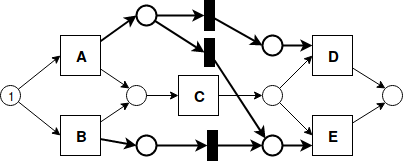
\includegraphics[width=\textwidth]{figures/algorithm/LT_Seq_01_Silent_01.png}
		\label{fig:seq-2-silent-1}
		\caption{For situation 2}
	\end{subfigure}
	\hfill
	\begin{subfigure}[b]{\textwidth}
		\centering
		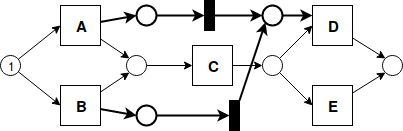
\includegraphics[width=\linewidth]{figures/algorithm/LT_Seq_01_Silent_03.png}
		\label{fig:seq-2-silent-2}
		\caption{For situation 4}
	\end{subfigure}
	\hfill
	\begin{subfigure}[c]{\textwidth}
		\centering
		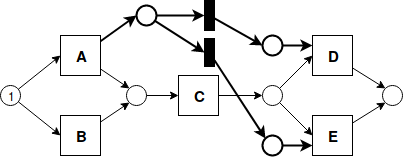
\includegraphics[width=\linewidth]{figures/algorithm/LT_Seq_01_Silent_02.png}
		\label{fig:seq-2-silent-3}
		\caption{For situation 5}
	\end{subfigure}
	\label{fig:seq-2-silent-cases}
	\caption{Silent Events for Long-term Dependency}
\end{figure} 

\subsection{Feasible cases due to soundness}
However, only with data from positive and negative information on the long-term dependency, it is possible to result in unsound model, because  some directly-follows relations about xor branches can be kept due to the existing model. When those relations do not show in the positive event log or shows only in negative event log, we get incomplete information and no evidence of long-term dependency is shown on those xor branches. In this way, it results in an unsound model, since those xor branches can't get fired to consume the tokens generated from the choices before.

For situation 1, it's full connected and xor branches can be chosen freely. So there is no need to add explicit connection on model to represent long-term dependency, therefore the model keeps same as original. 
For Situation 2 and 3, if $LT_S = XORB_S, LT_T= XORB_T$, then we can create an sound model by adding silent transitions. If not, then we need to use the duplicated transitions to create sound model. But before, we need to prove its soundness. 
For situation 4, 5 and 6, there is no way to prove the soundness even by adding duplicated events.

By adding constraints, we make sure only situations 1,2,3 happen when adding long-term dependency. 
\section{Reduce Silent Transitions}
%% We reduce the silent transition when there is no 
Our method to represent long-term dependency  can introduce redundant silent transitions and places. On one hand, it complicates the model; on the other hand, it causes the model unsound where the extra silent transitions suspend the execution and therefore violates the soundness condition of proper completion. So, in this step, we postprocess the Petri net to reduce silent transitions.
\begin{proposition}
	Given a silent transition $\epsilon$ in Petri net with input place set $P_{in}$ and output place set $P_{out}$, if $\vert P_{in} \vert \geq 2 \quad and \quad \vert P_{in} \vert \geq 2 $, the silent transitions can not be deleted. Else, the deletion is ok, and it does not damage the process model.
\end{proposition}
%% here we need to prove this proposition
One example is given in the following graph. 
\begin{figure}[!h]
	\centering
	\begin{subfigure}[a]{\textwidth}
		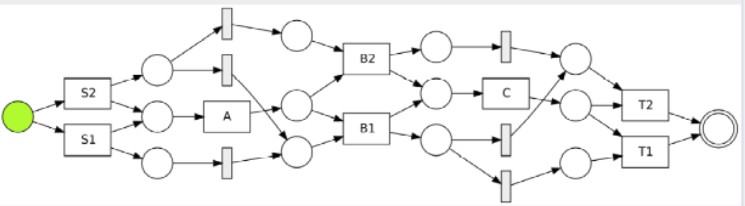
\includegraphics[width=\textwidth]{figures/algorithm/dfg-IM-pn-with-lt.png}
		\label{fig:with-lt}
		\caption{A Petri net with redundant silent transitions}
	\end{subfigure}
	\hfill
	\begin{subfigure}[b]{\textwidth}
		\centering
		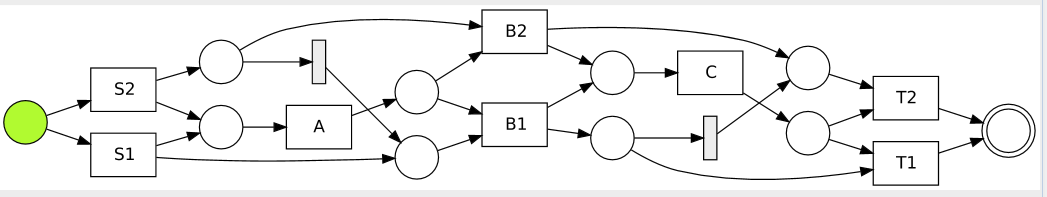
\includegraphics[width=\linewidth]{figures/algorithm/dfg-IM-pn-with-lt-reduced.png}
		\label{fig:reduced-lt}
		\caption{A Petri net with reduced silent transitions}
	\end{subfigure}
\end{figure}

